\section{Proofs and certificates}
\label{app:proofs}

\subsection{Theorem~\ref{thm:onebit}, in full}
\label{app:onebit}

Throughout, $n$ is odd, $S$ is uniform on $\cube$, $K = 2$, and a
\emph{reconstruction pair} is $(a,b) \in \cube \times \cube$ with label $0$
decoded to $a$ and label $1$ to $b$. Write
\[
  \Delta_{a,b}(s) \;=\; \dH(s,b) - \dH(s,a),
\]
and for a real $x$ put $x^+ = \max(x,0)$ and $x^- = \max(-x,0)$.

\paragraph{Step 1: the record is one function, and each agent gets an orientation.}
For $K = 2$ the record is determined by $\enc(s) = \Prob(Y = 1 \mid S = s)$. The
deviation vector has two coordinates summing to zero,
$d_i(\sminus) = \bigl(-\delta_i(\sminus),\, \delta_i(\sminus)\bigr)$ with
$\delta_i(\sminus) = \enc(1,\sminus) - \enc(0,\sminus)$, so for any bounded
$\pay_i \in [0,1]^2$,
\[
  \langle \pay_i, d_i(\sminus)\rangle
  \;=\; \bigl(\pay_i[1] - \pay_i[0]\bigr)\,\delta_i(\sminus),
  \qquad \bigl|\pay_i[1]-\pay_i[0]\bigr| \le 1 .
\]
Hence \eqref{eq:margin} holds for agent~$i$ if and only if there is a sign
$\sigma_i \in \{\pm 1\}$ with $\sigma_i\,\delta_i(\sminus) \ge \gamma$ for every
$\sminus$; the optimal decoder is $\pay_i[1]-\pay_i[0] = \sigma_i$.

\paragraph{Step 2: aligning the orientations, and the range of $\gamma$.}
Let $T = \{i : \sigma_i = -1\}$ and replace $\enc$ by
$\tilde\enc(s) = \enc(s \oplus \mathbf{1}_T)$ and $(a,b)$ by
$(a \oplus \mathbf{1}_T,\, b \oplus \mathbf{1}_T)$. The uniform prior is
invariant under $s \mapsto s \oplus \mathbf{1}_T$ and Hamming loss is
equivariant, $\dH(s \oplus \mathbf{1}_T, \hat s \oplus \mathbf{1}_T) = \dH(s,\hat s)$,
so $D$ is unchanged while every orientation becomes $+1$. We may therefore assume
\begin{equation}
  \enc(s + e_i) - \enc(s) \;\ge\; \gamma \qquad \text{for all } s \text{ and } i .
  \label{eq:aligned}
\end{equation}
Writing $\enc(s) = \gamma|s| + r(s)$, condition~\eqref{eq:aligned} says exactly
that $r$ is nondecreasing on the cube, and $\enc \in [0,1]$ together with
monotonicity forces $r(0^n) \ge 0$ and $r(1^n) \le 1 - n\gamma$, i.e.
\begin{equation}
  r \text{ monotone}, \qquad 0 \;\le\; r \;\le\; 1 - n\gamma .
  \label{eq:cone}
\end{equation}
In particular the feasible set is empty once $n\gamma > 1$: chaining
\eqref{eq:aligned} along a maximal path gives
$\enc(1^n) - \enc(0^n) \ge n\gamma > 1$, impossible for $\enc \in [0,1]$. This is
the final clause of Theorem~\ref{thm:onebit}.

\paragraph{Step 3: fix the reconstruction pair \emph{before} averaging.}
Under \emph{optimal} decoding $D(\enc) = \min_{a,b} D(\enc;a,b)$ is a minimum of
linear functionals of $\enc$ and hence \emph{concave}, so replacing $\enc$ by its
$S_n$-average can only \emph{increase} it---the wrong direction for a lower
bound. We therefore fix $(a,b)$ first and keep it fixed through Step~4. (This is
the proof-order correction discussed in Section~\ref{sec:onebit}; the argument
below then needs no averaging step at all.)

\begin{lemma}[Splitting]
\label{lem:split}
For every $\enc$ and every pair $(a,b)$,
$D(\enc;a,b) = \tfrac{n}{2} + \E\bigl[\enc(S)\,\Delta_{a,b}(S)\bigr]$.
\end{lemma}

\begin{proof}
$D(\enc;a,b) = \E\bigl[(1-\enc(S))\dH(S,a) + \enc(S)\dH(S,b)\bigr]
 = \E[\dH(S,a)] + \E[\enc(S)\Delta_{a,b}(S)]$, and $\E[\dH(S,a)] = n/2$ for
every $a$, since each coordinate disagrees with $a_i$ with probability $1/2$.
\end{proof}

\paragraph{Step 4: the exact minimum for a fixed pair.}
Substituting $\enc = \gamma|s| + r$ into Lemma~\ref{lem:split},
\[
  D(\enc;a,b) \;=\; \tfrac{n}{2}
   + \gamma\,\E\bigl[|S|\Delta_{a,b}(S)\bigr]
   + \E\bigl[r(S)\Delta_{a,b}(S)\bigr].
\]
Only the last term involves $r$, and by \eqref{eq:cone} we have
$0 \le r \le 1-n\gamma$ pointwise, so term by term
\begin{align*}
  \E\bigl[r(S)\Delta_{a,b}(S)\bigr]
  &\;\ge\; (1-n\gamma)\,\E\bigl[\min(\Delta_{a,b}(S),0)\bigr] \\
  &\;=\; -(1-n\gamma)\,\E\bigl[\Delta_{a,b}(S)^-\bigr],
\end{align*}
valid because $\gamma \le 1/n$. Hence, for every pair,
\begin{multline}
  \min_{\enc \text{ feasible}} D(\enc;a,b) \;\ge\;
  \tfrac{n}{2} + \gamma\,\E\bigl[|S|\Delta_{a,b}(S)\bigr] \\
  {} - (1-n\gamma)\,\E\bigl[\Delta_{a,b}(S)^-\bigr]
  \;=:\; L(a,b).
  \label{eq:LB}
\end{multline}
Only the \emph{box} part of \eqref{eq:cone} was used here; monotonicity enters
once, at the end of Step~5, to show the bound is attained.

\paragraph{Step 5: minimising over reconstruction pairs, for general $n$.}
Partition the coordinates by the pair: let
$A_{01} = \{i : a_i = 0, b_i = 1\}$ and $A_{10} = \{i : a_i = 1, b_i = 0\}$, with
$p = |A_{01}|$ and $m = |A_{10}|$, so $p + m \le n$. Coordinates with $a_i = b_i$
contribute equally to both distances and drop out:
\begin{equation}
  \Delta_{a,b}(s) \;=\; \sum_{i \in A_{01}} (1 - 2s_i)
                     \;-\; \sum_{i \in A_{10}} (1 - 2s_i).
  \label{eq:delta}
\end{equation}

\begin{lemma}[First moment]
\label{lem:firstmoment}
$\E\bigl[|S|\,\Delta_{a,b}(S)\bigr] = -\tfrac{1}{2}(p-m)$.
\end{lemma}

\begin{proof}
$\E[s_j(1-2s_i)] = 0$ for $i \ne j$ by independence, and
$\E[s_i(1-2s_i)] = \E[s_i - 2s_i] = -\tfrac12$ because $s_i^2 = s_i$. Summing
\eqref{eq:delta} over the two blocks gives $-\tfrac12 p + \tfrac12 m$.
\end{proof}

\begin{lemma}[Rademacher coupling]
\label{lem:rademacher}
Let $R_k$ denote a sum of $k$ independent Rademacher variables. Then
$\E\bigl[\Delta_{a,b}(S)^-\bigr] = \tfrac12\,\E\bigl|R_{p+m}\bigr|$, and
$k \mapsto \E|R_k|$ is nondecreasing.
\end{lemma}

\begin{proof}
By \eqref{eq:delta}, $-\Delta_{a,b}(S) = X - Y$ where
$X = \sum_{i \in A_{01}}(2s_i - 1)$ and $Y = \sum_{i \in A_{10}}(2s_i - 1)$ are
independent sums of $p$ and of $m$ independent Rademacher variables. As $Y$ is
symmetric, $X - Y$ has the law of $R_{p+m}$, so
$\E[\Delta^-] = \E[(X-Y)^+] = \E[R_{p+m}^+] = \tfrac12\E|R_{p+m}|$, the last step
by symmetry of $R_{p+m}$. For monotonicity, condition on $R_k$ and apply Jensen
to the convex map $x \mapsto |x|$:
\[
  \E|R_{k+1}| = \E\bigl|R_k + \varepsilon_{k+1}\bigr|
  \;\ge\; \E\bigl|\E[R_k + \varepsilon_{k+1} \mid R_k]\bigr| = \E|R_k| . \qedhere
\]
\end{proof}

\begin{proposition}[The antipodal pair is optimal]
\label{prop:antipodal}
For every reconstruction pair $(a,b)$ and every $0 \le \gamma \le 1/n$,
\[
  L(a,b) \;\ge\; \Mn + n\gamma\Bigl(\tfrac{n-1}{2} - \Mn\Bigr),
\]
with equality for the antipodal pair $(a,b) = (0^n, 1^n)$.
\end{proposition}

\begin{proof}
Combining \eqref{eq:LB} with Lemmas~\ref{lem:firstmoment} and
\ref{lem:rademacher},
\[
  L(a,b) \;=\; \tfrac{n}{2} - \tfrac{\gamma}{2}(p-m)
  - (1-n\gamma)\,\tfrac12\E\bigl|R_{p+m}\bigr| .
\]
Two comparisons finish it. First, $p - m \le p + m \le n$ and $\gamma \ge 0$, so
$-\tfrac{\gamma}{2}(p-m) \ge -\tfrac{n\gamma}{2}$. Second, $p+m \le n$ and
$1 - n\gamma \ge 0$, so by the monotonicity in Lemma~\ref{lem:rademacher},
$-(1-n\gamma)\tfrac12\E|R_{p+m}| \ge -(1-n\gamma)\tfrac12\E|R_n|$. Therefore
\[
  L(a,b) \;\ge\; \tfrac{n}{2} - \tfrac{n\gamma}{2}
              - (1-n\gamma)\tfrac12\E|R_n| .
\]
Now $\min(|S|, n-|S|) = \tfrac12\bigl(n - \bigl|2|S|-n\bigr|\bigr)$ and
$R_n \overset{d}{=} 2|S| - n$, so $\tfrac12\E|R_n| = \tfrac{n}{2} - \Mn$, and
collecting terms turns the right-hand side into
$\Mn + n\gamma\bigl(\tfrac{n-1}{2} - \Mn\bigr)$.

For equality take $a = 0^n$ and $b = 1^n$, so $p = n$, $m = 0$ and
$\Delta(s) = n - 2|s|$, which is negative exactly on $\{|s| > n/2\}$ --- there
are no ties, as $n$ is odd. Both comparisons above are then equalities, and the
pointwise bound in \eqref{eq:LB} is attained by
\[
  r^\ast(s) \;=\; (1-n\gamma)\,\ind{|s| > n/2},
\]
which takes the value $1-n\gamma$ exactly where $\Delta < 0$ and $0$ elsewhere.
Being the indicator of an up-set, $r^\ast$ is monotone, so it satisfies
\eqref{eq:cone} and is feasible. Hence $L(0^n,1^n)$ is achieved by the record
$\enc^\ast(s) = \gamma|s| + (1-n\gamma)\ind{|s|>n/2}$.
\end{proof}

Proposition~\ref{prop:antipodal} gives both directions of
Theorem~\ref{thm:onebit}: no feasible record and reconstruction pair does better
than $\Mn + n\gamma(\frac{n-1}{2}-\Mn)$, and $\enc^\ast$ with antipodal decoding
attains it. With Step~2 covering $\gamma > 1/n$, the theorem follows.

\begin{remark}[What the proof does \emph{not} need]
\label{rem:notneeded}
No permutation averaging is used, so the concavity obstruction of Step~3 is
avoided rather than worked around; and no vertex description of the monotone
polytope is needed, since \eqref{eq:LB} uses only the box
$0 \le r \le 1-n\gamma$ and monotonicity is checked once, on $r^\ast$. The
$S_n$-orbit reduction to $\binom{n+3}{3}$ representatives indexed by
$(n_{00},n_{01},n_{10},n_{11})$ is therefore a computational convenience for the
verification in Table~\ref{tab:onebit}, not a step of the proof.
\end{remark}

\subsection{Lemma~\ref{lem:necessity} and Lemma~\ref{lem:gen-margin}}
\label{app:threshold}

\paragraph{Necessity.}
Let $\Dnull$ be strictly decreasing at $K$, so the $K$ centres are distinct, and
suppose some $s \notin C$ has a unique nearest centre $c$, at distance
$r = d(s,C) \ge 1$. Every other centre satisfies $d(s,c') \ge r+1$. Flip one bit
of $s$ towards $c$ to get $s'$: then $d(s',c) = r-1$, while
$d(s',c') \ge d(s,c') - 1 \ge r$ for every $c' \ne c$, so $c$ is again the unique
nearest centre of $s'$. Attaining $\Dnull(K)$ puts each profile's label mass on
its nearest centres, so $\enc[s,\cdot]$ and $\enc[s',\cdot]$ are both the point
mass on $\ell(c)$; the corresponding $d_i$ vanishes identically, and
$\langle \pay_i, d_i \rangle = 0$ for every $\pay_i \in [0,1]^K$. Iterating from
$s'$ reaches $c$, and the same argument applied at each radius reaches every
non-centre with a unique nearest centre. When $C$ is dominating this says
precisely that every $t \notin C$ has $|N(t) \cap C| \ge 2$, i.e.\ $C$ is
2-dominating.

\paragraph{Sufficiency, with the case analysis written out.}
Let $C$ be 2-dominating, $|C| = K$, and take
$\enc[c,\cdot] = \delta_{\ell(c)}$ for $c \in C$ and
$\enc[t,\cdot] = \mathrm{Unif}\bigl(\ell(N(t)\cap C)\bigr)$ for $t \notin C$,
with $\pay_i[y] = (\text{centre of } y)_i$.

\emph{Distortion.} Each label's Bayes reconstruction is its own centre. A centre
is reconstructed exactly; a non-centre puts all of its mass on centres at
distance $1$, so it costs exactly one bit. Hence $D = (2^n - K)/2^n$. Conversely
any record with $K$ labels reconstructs at most $K$ profiles exactly and pays at
least one bit on each of the rest, so $\Dnull(K) \ge (2^n-K)/2^n$; therefore
$D = \Dnull(K)$.

\emph{Margin.} Write $m_i(t) = \E_{y \sim \enc[t,\cdot]}\bigl[\pay_i[y]\bigr]$
for the average $i$-th bit of the centres $t$'s mass sits on, so that for an edge
$s_1 = s_0 + e_i$ we have
$\langle \pay_i, d_i \rangle = m_i(s_1) - m_i(s_0)$. Write
$d(t) = |N(t) \cap C| \ge 2$ for $t \notin C$. Four cases:
\begin{enumerate}
\item $s_0, s_1 \in C$: $m_i(s_0) = 0$ and $m_i(s_1) = 1$; margin $1$.
\item $s_0 \notin C$, $s_1 \in C$: $m_i(s_1) = 1$. The centre-neighbours of $s_0$
      are $s_1$, whose $i$-th bit is $1$, and vertices $s_0 + e_j$ with
      $j \ne i$, whose $i$-th bit equals $(s_0)_i = 0$. So $m_i(s_0) = 1/d(s_0)$
      and the margin is $1 - 1/d(s_0)$.
\item $s_0 \in C$, $s_1 \notin C$: symmetrically $m_i(s_0) = 0$ and
      $m_i(s_1) = 1 - 1/d(s_1)$; margin $1 - 1/d(s_1)$.
\item $s_0, s_1 \notin C$: every centre-neighbour of $s_1$ is some $s_1 + e_j$
      with $j \ne i$, because $s_0 \notin C$, and each has $i$-th bit
      $(s_1)_i = 1$, so $m_i(s_1) = 1$; symmetrically $m_i(s_0) = 0$; margin $1$.
\end{enumerate}
The worst case is case~2 or case~3 at a non-centre of minimum degree, so the
all-teammate-profile margin is exactly $1 - 1/\dmin \ge 1/2$. Neither argument
uses any property of $\pay_i$ beyond $\pay_i \in [0,1]^K$.

\subsection{Lemma~\ref{lem:shell}}

Fix a record with centre set $C$, $|C| = K$. A profile at distance $r$ from $C$
requires at least two centres at distance exactly $r$
(Lemma~\ref{lem:necessity}, applied at radius $r$). Each centre is at distance
$r$ from exactly $\binom{n}{r}$ profiles, so the number of (profile, centre)
incidences at radius $r$ is at most $K\binom{n}{r}$, and shell $r$ therefore
holds at most $\lfloor K\binom{n}{r}/2\rfloor$ profiles. Filling shells from the
inside minimises $\sum_s d(s,C)$ subject to those capacities, giving a lower
bound on $2^n \Dnull$; comparing it against $2^n - K$ excludes $(n,K)$.

\subsection{The smallest case, in full}

At $n = 3$ the optimal record is the odd-weight parity class,
$C = \{001, 010, 100, 111\}$, which is $2$-dominating with $\dmin = 3$
(Figure~\ref{fig:q3}). Each of the four even-weight profiles spreads its mass
uniformly over all three of its neighbours, every label is a centre, the
reconstruction errs by exactly one bit on half the profiles---so
$D = \Dnull(4) = 1/2$---and the margin is $1 - 1/3 = 2/3$.

The parity class is $2$-dominating in every dimension, giving
$\gtwo(\Qn) \le 2^{\,n-1}$ --- which is also what Bujt'{a}s and
Jask'{o}'s~\cite{bujtasjasko} bound $\gtwo(G) \le |V|/2$ for $\delta(G) \ge 3$
gives on $\Qn$, and we claim no credit for it; it is optimal only at $n = 3$, where
$2^{\,n-1} = 4$ happens to meet the Fink--Jacobson bound.

\begin{figure}[t]
\centering
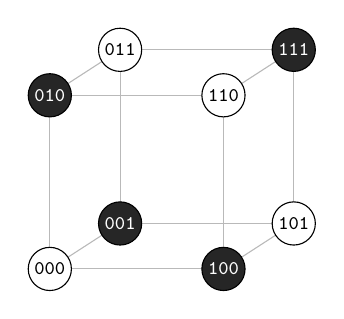
\begin{tikzpicture}[scale=1.05,
  ctr/.style={circle, draw, fill=black!85, text=white, inner sep=1.4pt,
              font=\scriptsize\ttfamily},
  non/.style={circle, draw, fill=white, inner sep=1.4pt,
              font=\scriptsize\ttfamily},
  ed/.style={gray!55}]
  % cube coordinates: back face offset
  \def\dx{0.85}\def\dy{0.55}
  \coordinate (c000) at (0,0);
  \coordinate (c100) at (2.1,0);
  \coordinate (c010) at (0,2.1);
  \coordinate (c110) at (2.1,2.1);
  \coordinate (c001) at (\dx,\dy);
  \coordinate (c101) at (2.1+\dx,\dy);
  \coordinate (c011) at (\dx,2.1+\dy);
  \coordinate (c111) at (2.1+\dx,2.1+\dy);
  \foreach \a/\b in {c000/c100, c000/c010, c100/c110, c010/c110,
                     c001/c101, c001/c011, c101/c111, c011/c111,
                     c000/c001, c100/c101, c010/c011, c110/c111}
    \draw[ed] (\a) -- (\b);
  \node[non] at (c000) {000};
  \node[ctr] at (c100) {100};
  \node[ctr] at (c010) {010};
  \node[non] at (c110) {110};
  \node[ctr] at (c001) {001};
  \node[non] at (c101) {101};
  \node[non] at (c011) {011};
  \node[ctr] at (c111) {111};
\end{tikzpicture}
\caption{$\Kflat(3) = \gtwo(Q_3) = 4$. Filled vertices are the record's four
centres---the odd-weight parity class. Every non-centre has all three of its
neighbours in $C$, so $\dmin = 3$ and the margin is $2/3$.}
\label{fig:q3}
\end{figure}

\subsection{Reproducing every number in this paper}
\label{app:repro}

\begin{verbatim}
python run.py verify   # integrity, then the checks
python run.py audit    # printed numbers vs artifacts
python run.py score    # pre-registered predictions
python run.py figures  # regenerate every figure

# the only step needing a solver, run once:
python src/make_certificates.py
\end{verbatim}

\noindent
\texttt{verify\_all.py} is an independent reimplementation: it rebuilds
$\gtwo(\Qn)$ for $n \le 4$ by complete enumeration of all $2^{2^n}$ subsets,
rechecks every certified code for $2$-domination from scratch, constructs the
record of Lemma~\ref{lem:gen-margin} explicitly and evaluates its distortion and
its all-teammate-profile margin by direct enumeration, re-derives the shell
exclusions, compares the one-bit record against the closed form of
Theorem~\ref{thm:onebit}, and checks every step of
Proposition~\ref{prop:antipodal}---the Rademacher identity and its monotonicity,
the bound \eqref{eq:LB} over all $4^n$ reconstruction pairs at $n = 3,5$ and over
all $(p,m)$ orbits at $n = 7,9$, and feasibility of $r^\ast$. It recomputes every
cell of Table~\ref{tab:ratio} from the two bounds on $\gtwo(\Qn)$, and it checks
the counterexamples of Section~\ref{sec:threshold} by direct enumeration: at
$n = 3,4$ under the Bernoulli$(0.7)$ prior it enumerates every $K$-subset,
identifies the $\pi$-optimal codes, and exhibits a flat record with
$D = \Dnull(K)$ and $\gamma > 0$ at a $K$ below the withdrawn threshold. All $99$ checks pass in the pinned environment (Python 3.10.11, NumPy 2.2.6, SciPy
1.15.3).

\paragraph{A correction, and what it says about our verification.}
An earlier version of this paper claimed a general-prior threshold of
$2^n - (n-1)$. It was wrong, and the way it was wrong is worth recording. Both
verification routes---the solver-free checks and the independent
\texttt{prior\_threshold.py} MILP---searched for a \emph{2-dominating} set, so
both encoded the same incorrect reading of Lemma~\ref{lem:necessity}. They
agreed on $6$, $28$ and $122$ at $n = 3,5,7$, and their agreement was worth
nothing, because independence of implementation does not buy independence of
specification. The error was caught by a test that asked a different
question---relax $\gamma$ and ask an LP directly whether $\Dnull(K)$ is
attainable---rather than by a second implementation of the same question.

The MILP-derived facts---infeasibility of $2$-domination at $(n,K) = (5,9)$,
$(7,29)$, $(7,30)$, $(7,31)$, $(9,94)$, $(9,95)$ and $(9,96)$---are the only
claims that require a solver, and each is a proved-infeasible status rather than
a time limit. Infeasibility admits no small witness, so these are the only claims
the solver-free verifier cannot recheck; the $n=9$ rows were re-proved in the
pinned environment by \texttt{gamma2\_n9\_lb\_rerun.py}.

\paragraph{Theorem~\ref{thm:prior}, machine-checked.}
The three load-bearing claims---the edge structure of
Lemma~\ref{lem:edge-structure}, the strict descent of
Lemma~\ref{lem:strict-descent}, and the closed form of
Lemma~\ref{lem:gen-margin} against the Theorem~\ref{thm:elim} LP---were checked
on all $47{,}017$ $\pi$-optimal codes at $n \le 4$ over eight product priors, by
exhaustive search over \emph{every} code at $n = 3,4$ and over every
radius-$\ge 2$ configuration at $n = 5$ (vertex-transitivity and coordinate
permutation place the bad edge at $(0^n, e_1)$, reducing $2^{32}$ codes to
$724{,}566$), and on $20{,}000$ random codes at $n \le 7$, of which $8{,}517$
satisfy the hypothesis of Lemma~\ref{lem:strict-descent} and all $8{,}517$
satisfy its conclusion. No violation of any kind was found. We note that the
first run of this check \emph{failed}, correctly: an earlier draft of
Lemma~\ref{lem:edge-structure} applied fixed-centre parity to the distance to the
\emph{set}, and the harness rejected it at $n=3$, $K=2$ rather than passing
silently.

\paragraph{The registered predictions, counted.}
$22$ predictions were registered and hashed before each harness was written. $5$
were registered as derivations---predictions whose failure would mean a theorem
or the code was wrong. One of those, that a sampled run reproduces the exact
enumeration, we re-graded to uncertain \emph{before} scoring, because convergence
of an empirical encoder is a statistical claim and not a derivation; that leaves
$4$, and all $4$ held. Of the remaining $18$, $10$ were falsified, $7$ were
confirmed, and $1$ was not scoreable because it referred to a task design we
replaced before running it. Every falsification is reported as a falsification,
here and in the sections above.
